\documentclass{standalone}
\usepackage{tikz} % Import the tikz package
\usetikzlibrary{automata} % Import library for drawing automata
\usetikzlibrary{positioning} % ...positioning nodes
\usetikzlibrary{arrows} % ...customizing arrows
\tikzset{node distance=2.5cm,
    every state/.style={
        semithick,
        fill=gray!10},
    initial text={},
    double distance=2pt,
    every edge/.style={
        draw,
        ->,>=stealth',
        auto,
        semithick}}
\let\epsilon\varepsilon
\begin{document}
    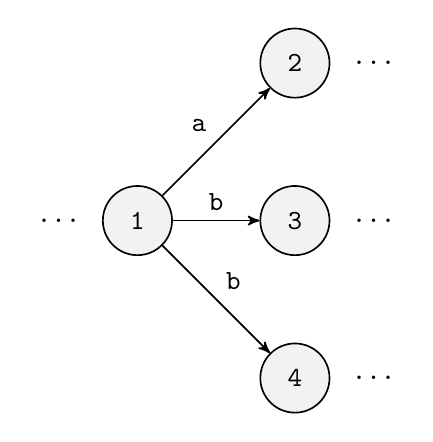
\begin{tikzpicture}
        \node (ldots1) at (0,0) {\tt \ldots};
        \node[state] (1) at (1,0) {\tt 1};
        \node[state] (2) at (3,2) {\tt 2};
        \node[state] (3) at (3,0) {\tt 3};
        \node[state] (4) at (3,-2) {\tt 4};
        \node (ldots1) at (4,2) {\tt \ldots};
        \node (ldots1) at (4,0) {\tt \ldots};
        \node (ldots1) at (4,-2) {\tt \ldots};

        \draw (1) edge[] node {\tt a} (2);
        \draw (1) edge[] node {\tt b} (3);
        \draw (1) edge[] node {\tt b} (4);
    \end{tikzpicture}
\end{document}